\chapter{Membrane potential heterogeneity at the mitochondrial network level}\label{ch:five}
\clearpage
\section{Introduction}
Mitochondria in yeast form a tubular network along the inner periphery of the cell. The mitochondrial network undergoes dynamic remodeling by fission and fusion events. The function and mechanisms of these remodeling events have been an active research field for the last two decades \cite{hoitzing_what_2015}. The proteins that play an essential role in mitochondrial fission and fusion dynamics belong to the Dynamin family. In yeast, the key proteins are MGM1, FZO1 and DNM1. MGM1 (OPA1 in mammalian cells) mediates inner mitochondrial membrane fusion, FZO1 (mitofusin MFN1 and MFN2 in mammalian cells) mediates outer mitochondrial membrane fusion while DNM1 (DRP1 in mammalian cells) mediates fission. Fission and fusion rates are balanced \cite{shaw_mitochondrial_2002}. Deletion or knockdown of fusion related proteins result in a highly fragmented network while deletion of fission proteins result in a highly branched, 'net-like' structure \cite{shaw_mitochondrial_2002}. Inhibition of fusion and fission results in a host of cellular defects resulting from OXPHOS deficiencies, mtDNA loss and increased ROS production \cite{chen_disruption_2005,ishihara_regulation_2006,nunnari_mitochondria:_2012}. In humans, mutations in the fusion related proteins MFN2 and OPA1 result in mitochondrial and neurodegenerative diseases such as Charcot Marie Tooth, dominant optic atrophy (DOA), Parkinson's and Alzheimer's disease \cite{alexander_opa1_2000,bliek_mechanisms_2013,wang_impaired_2009}.

The severe consequences of the loss of mitochondrial fusion related proteins imply that mitochondrial fission and fusion dynamics is tightly integrated with cellular bioenergetics \cite{sauvanet_energetic_2010}. Fusion promotes a connected network which is hypothesized to mediate faster and more effective mixing of mitochondrial proteins \cite{busch_quality_2014,wilkens_restricted_2013}. A fused mitochondrial network has also been hypothesized to mediate an increase in ATP production via several pathways including changes to the cristae curvature \cite{patten_opa1-dependent_2014}, decrease in proton leak \cite{gnaiger_mitochondrial_2002} and by serving as a transmission power cable \cite{amchenkova_coupling_1988}. This transmission power cable hypothesis says that fused mitochondrial networks enable the electrochemical gradient from one end of the network to be used at another end. Mitochondrial dynamics are required for mitochondrial quality control \cite{twig_fission_2008}. In this process, a healthy mitochondrial network is maintained by segregation/fission of mitochondrial fragments from the network and selective fusion of those fragments back to the network. Selective fusion means that only fragments above a certain quality threshold (as measured by mitochondrial membrane potential, ΔΨ) can fuse back to the network \cite{legros_mitochondrial_2002,meeusen_mitochondrial_2004}. Because healthy mitochondria are more likely to fuse to the network, most of the observed isolated fragments of mitochondria will be those that are unhealthy/below the threshold for ΔΨ. Fission can be thought of as a way for the network to protect itself from unhealthy mitochondrial fragments. According to the mitochondrial quality control model, isolated mitochondrial fragments that are unable to fuse back to the network are targeted for degradation by the autophagic machinery, a process know as mitophagy.
%
\begin{figure}[htp]
	\centering
    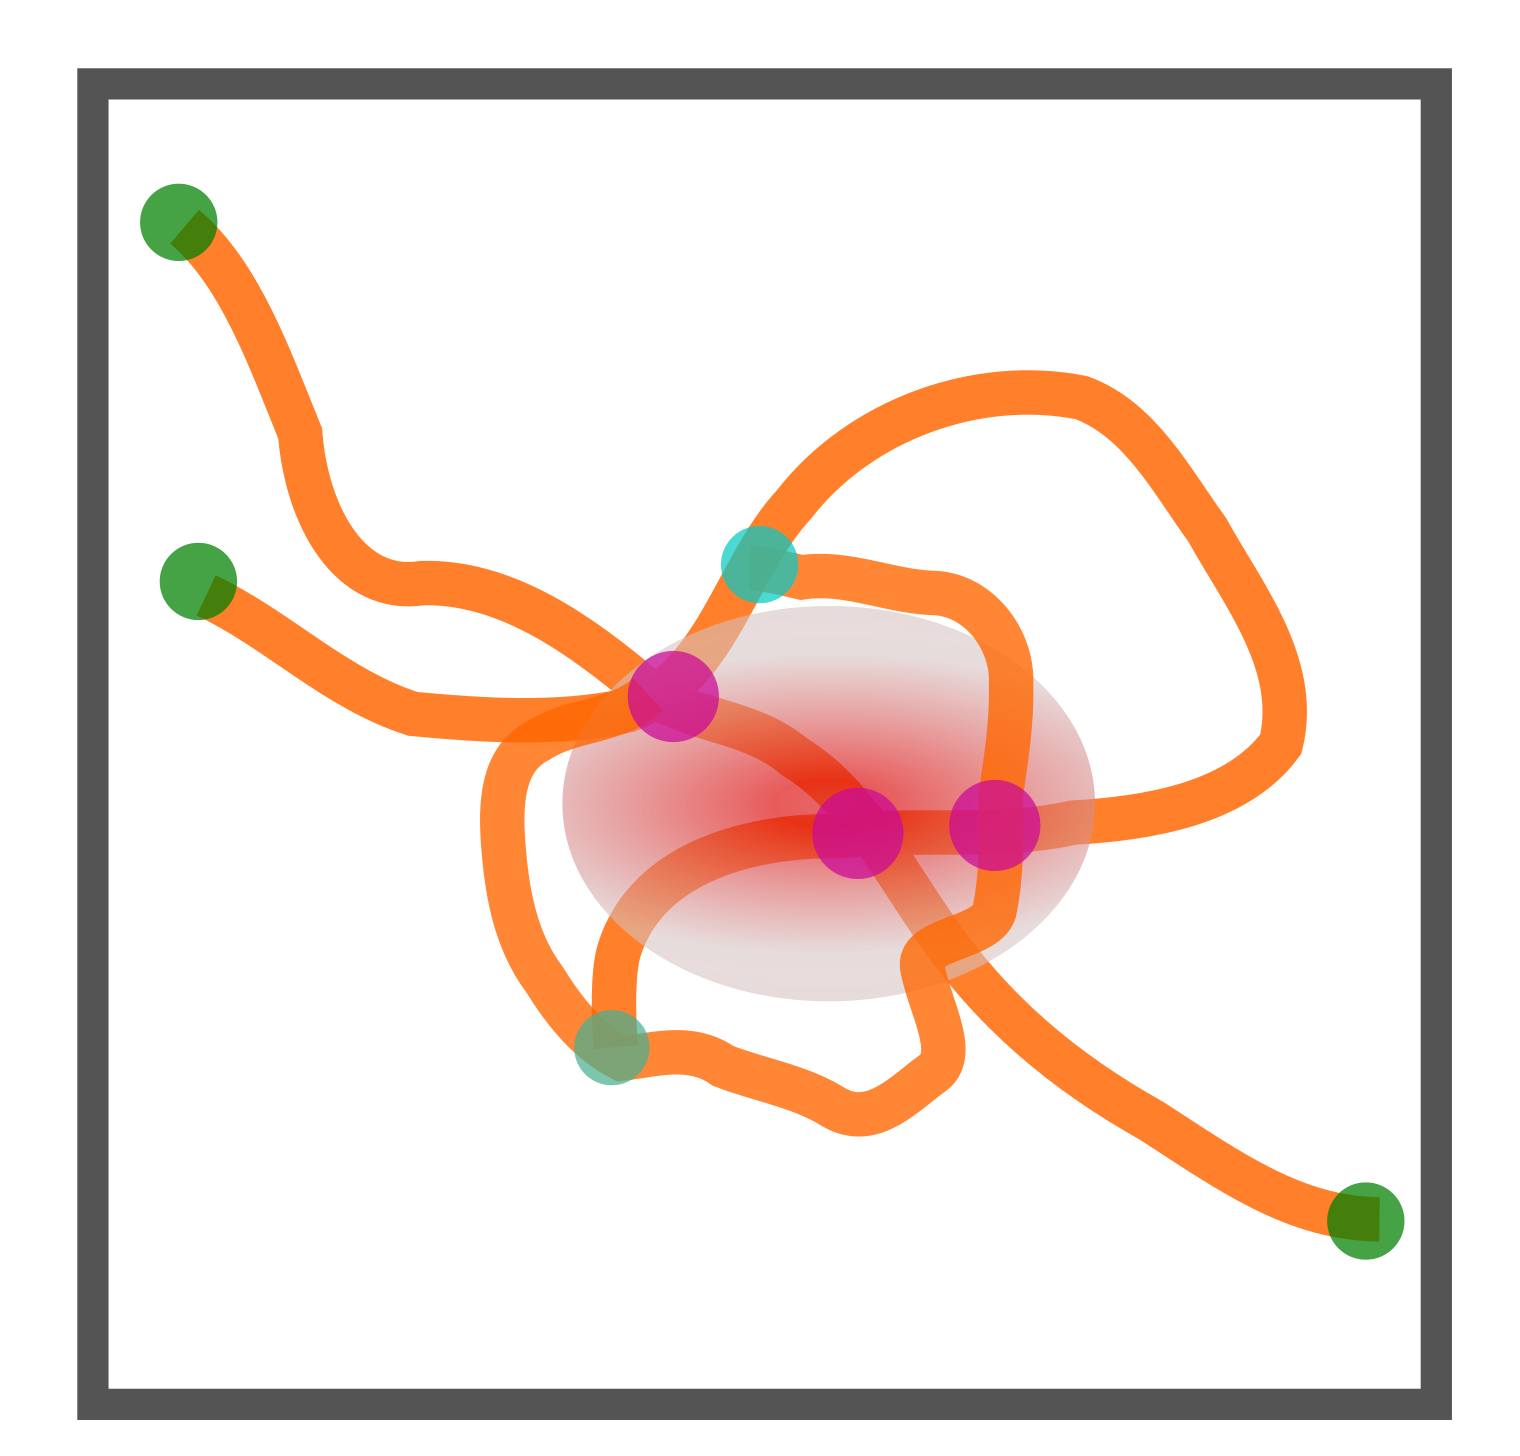
\includegraphics[width=.5\textwidth]{cartoon}
    \caption[Heterogeneity of structure-function in mitochondrial networks]{Heterogeneity of structure-function in mitochondrial networks.\\Shown here is a region of a mitochondrial network within a yeast cell. Branchpoints representing the intersection of mitochondrial tubules are shown as the cyan and magenta nodes. The area in red is a region of high connectivity because the magenta nodes have a higher degree of connectivity (they are connected to more connected nodes) compared to the cyan and green nodes. Our hypothesis is that these sites are enriched for ΔΨ based on the increased rate of fusion events occurring in these regions.}\label{fig:cartoon}
\end{figure}
%

Mitochondrial quality control via fission and fusion dynamics imply some level of heterogeneity in the distribution of ΔΨ within the network. Functional complementation through fusion based mixing and segregation of unhealthy mitochondria through fission would be unnecessary if mitochondrial quality (as indicated by ΔΨ) was homogeneous throughout the network. Previous studies have relied on qualitative descriptions of changes in mitochondrial morphology when undergoing a change in respiration states \cite{jakobs_spatial_2003,sesaki_division_1999}. They did not directly quantify the relationship between the topology of the mitochondrial network and its functional state. In this chapter we investigate the relationship between mitochondrial network structure (topology/connectivity) and functional heterogeneity (ΔΨ) in mitochondrial networks, i.e. whether structural features of regions within the network is indicative of the bioenergetic state of that region (\Fref{fig:cartoon}). 

The first area that we investigate is the relationship between mitochondrial network connectivity and the density of mitochondrial tubules at the cell surface. We define surface density as a measure that represents how 'packed' with mitochondrial tubules a given cell surface is. We expect that network connectivity should scale with surface density of the network, because mitochondrial tubules in denser networks would have a higher probability of encountering and fusing with another tubule. In addition we expect to see a clear difference between mitochondrial networks in fermentation and respiratory conditions. When yeast cells are grown in a non-fermentable substrate, the mitochondrial volume as a proportion of cell volume (volume ratio) increases dramatically \cite{jakobs_spatial_2003}. Mitochondria in glucose (fermentation) form very simple networks, with few branching points, while mitochondria in glycerol (respiration inducing) form networks that are more branched and elaborate \cite{egner_fast_2002}. We investigate the connectivity at the global (whole cell) and local (part of the cell) level in response to changes in surface density brought about by cells growing in different carbon sources (details in \fref{sec:carbon}).  We also expect to see a difference in the connectivity measures of mitochondrial networks grown in the three different respiration inducing carbon sources (lactate, glycerol+ethanol and raffinose) based on their overall oxygen consumption rate (OCR) and ΔΨ levels (\Fref{fig:O2dy}). 

The second area we investigate is the relationship between surface density, network connectivity and mitochondrial membrane potential (ΔΨ). We hypothesize that surface density should scale with ΔΨ. Since respiratory conditions induce a change in volume ratio and surface density of mitochondria in a cell, and respiration requires ΔΨ, we expect that there will be some sort of relationship between the surface density of mitochondria and the overall level of ΔΨ. Furthermore, it has been suggested by observation that conditions that result in highly connected networks tend to favor more fission and fusion events \cite{jakobs_spatial_2003}. Therefore we hypothesize that ΔΨ scales with mitochondrial network connectivity. This is due to the selective fusion mechanism where only mitochondria that are functional/healthy can fuse back to the network. 

We also investigate specific regions of the mitochondrial network known as branching points. These are the intersections of tubules within the network (\Fref{fig:cartoon}, red and cyan dots). Branching points are by definition sites of higher connectivity compared to non branching point regions. Therefore on average, more fusion events might take place in these regions, and therefore by the selective fusion principle they might display a higher ΔΨ level. Therefore we hypothesize that branching points within a network might have a higher level of ΔΨ compared to the rest of the network.

Lastly, we investigate the ΔΨ levels of isolated fragments of mitochondria. Based on the mitochondrial quality control model that says that isolated fragments of mitochondria that are unable to fuse back to the network are targeted for mitophagy, we expect these fragments to have a lower level of ΔΨ compared to the network. Furthermore because mitophagy selection is size dependent (i.e. only fragments below a certain size can undergo mitophagy) \cite{kanki_mitophagy_2008,rambold_tubular_2011} we expect smaller isolated fragments to have a lower ΔΨ compared to longer isolated fragments.
%
\begin{figure}[htp]
	\centering
    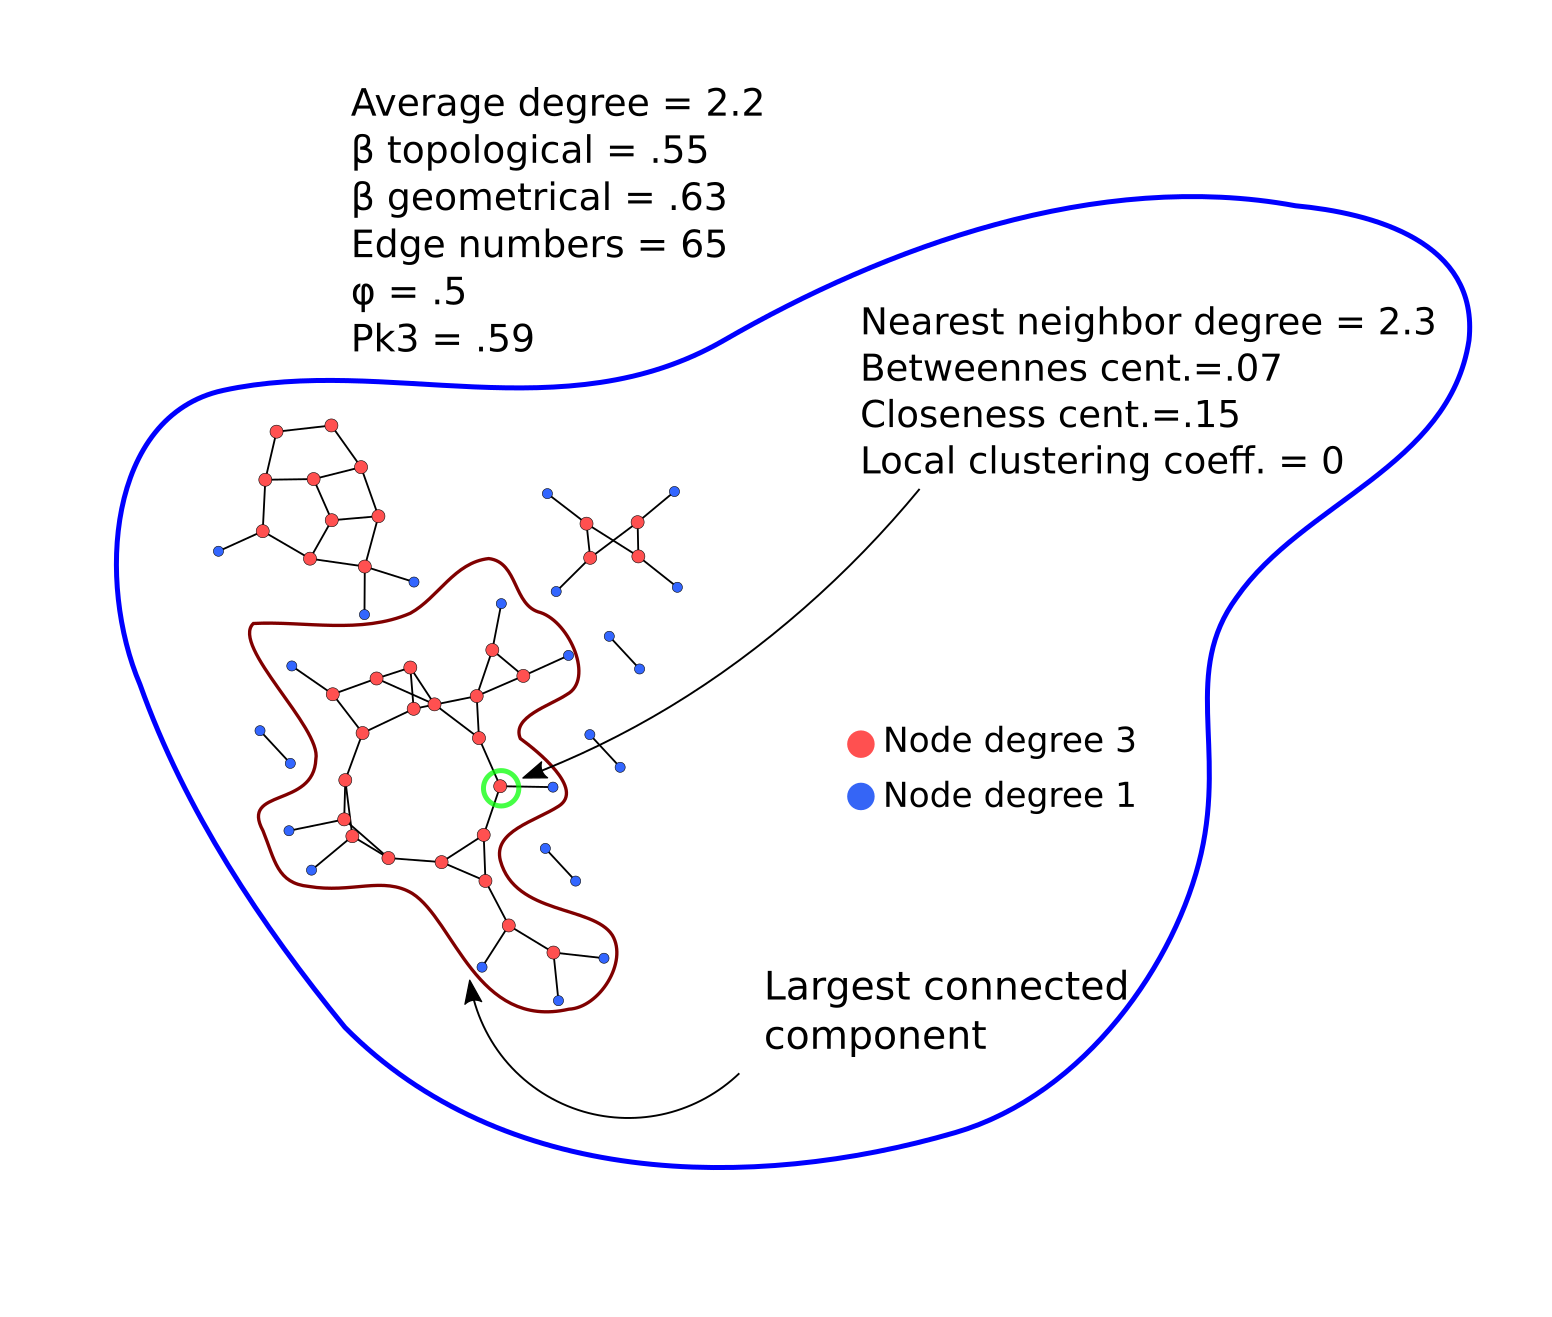
\includegraphics[width=.95\textwidth]{graph}
    \caption[Global and local connectivity in mitochondrial networks]{Global and local connectivity in mitochondrial networks.\\Shown here is a graph representation of a real mitochondrial network. Branching points representing the intersection of edges/tubules in the network are shown as red nodes, while the ends of the tubules are shown as blue nodes. The largest connected component circled in red is the largest completely connected entity in the graph. The measures outside the blue outline represent the global connectivity measures of the entire network/graph (area circled in blue). Global connectivity gives an overall measure of how interconnected the network is. The measures inside the blue outline represent the local connectivity measures of the network. Local connectivity measures shows the connectivity related to a region of the graph, hence they are tied to a particular node in the graph, for e.g. the local connectivity numbers shown are for the node circled in green.}\label{fig:graph}
\end{figure}
%
\section{Materials and Methods}
\subsection{Data structure}
The data calculated in this chapter utilizes the database structure as detailed in \fref{sec:database}. It consists of structural (area, length, volume), topological (network connectivity measures) and functional parameters (respiration, ΔΨ levels) organized at a per tubule, per cell and per population (carbon source) level. This allows analysis to be carried out at the scale appropriate to each question. For most of this chapter data is considered at the per cell level. However when we investigate branchpoint heterogeneity we query at the per tubule level since we interrogate the regions around a branchpoint, which consists of intersecting tubules. 

In this chapter we consider each mitochondrial network of a cell to be a planar, undirected graph. A planar graph is a graph that can be embedded in a plane, which means it can be drawn within a plane such that no edges cross each other \cite{west2001introduction}. A graph (\Fref{fig:graph}) has edges (corresponding to the tubules of a mitochondrial network) and nodes (corresponding to the ends of the individual tubules). The graphs were derived from the VTK spatial information output of MitoGraph v2.0 using the NetworkX (\url{https://networkx.github.io/}) module in Python. If a measure was specified as topological, each edge was considered to have a length of one (i.e. an unweighted graph). If a measure was specified as geometric, the edges of the graph had a weight equal to the real spatial length (in microns) of the tubule it represented.
 
\subsection{Surface density as a measure of spatial density of mitochondria}
Spatial density of mitochondria is a measure of how densely a mitochondrial network fills a given space. It can be expressed as volume ratio \cite{rafelski_mitochondrial_2012}, which is the proportion of the volume of the cell that consists of the mitochondrial network or it can be given as the surface density.
Volume ratio is appropriate when one is concerned only with the amount of mitochondria in a cell, for example when normalizing OCR to mitochondrial content. However in the context of this chapter where we are concerned with how the spatial density of mitochondria on the cell surface affects the connectivity of the network, surface density if more appropriate.  

The surface area $S$ of a cell which we assume is in the shape of a prolate ellipsoid ($a=b, c >a$, where $a$ is the minor axis and $c$ the major axis of the ellipsoid) is given by the formula \cite{olver_nist_2010}:
\begin{equation}
	\begin{split}
		\begin{aligned}
			S&=2\pi a^2 \left( 1+\frac{c}{ae} \arcsin(e)\right) \\[2ex]
			e&=\sqrt{1-\frac{a^2}{c^2}}
		\end{aligned}
	\end{split}
\end{equation}
We define the surface density of the mitochondrial network as:
\begin{equation}\label{eq:surfd}
	\begin{split}
		\begin{aligned}
			q&=\frac{L}{S}\\
			L&=\text{total length of mitochondrial network} \\
			S&=\text{surface area of cell}
		\end{aligned}
	\end{split}
\end{equation}
\subsection{Global and local measures of connectivity}
We use standard network theory terminology when defining measures of connectivity in the mitochondrial network, which we consider to be an undirected planar graph \cite{west2001introduction}. In this type of graph, the largest connected component is the largest subgraph with no unconnected /isolated edges (circled red in \Fref{fig:graph}). The degree of a node is defined as the number of edges connected to that node. For example, nodes at the ends of a graph have a degree of one. A branchpoint in our graph is a node with a degree of at least three. The average degree of all nodes in the network is often used as a standard measure of network connectivity.

\emph{Global Connectivity} measures are connectivity measures that relate to the whole network. These measures include:
\begin{equation}
	\begin{split}
		\begin{aligned}
			& \text{φ}=\text{Fraction of nodes in the largest connected component} \\
			&\text{β}_{\V{geometric}} = \text{Fraction of edges in largest connected component}\\
			&\text{β}_{\V{topological}} = \text{Fraction of total length of the largest connected component}\\
			& \mathrm{Pk_3} =\text{Fraction of nodes that have three edges}\\
			&\text{Network average degree} = 2\times \frac{\text{number edges}}{\text{number of nodes}}\\
			& \text{Number of edges in the graph}
		\end{aligned}
	\end{split}
\end{equation}
\emph{Local Connectivity} are measures that reflect the connectivity of specific regions within the network. These measures consist of:

\emph{Nearest neighbor degree} of a node is the average degree of all directly adjacent nodes. \\
\emph{Betweenness centrality} of node $v$ is given by \cite{brandes_faster_2001}:
\begin{equation}
	\begin{split}
		\begin{aligned}
			&B(v)=\displaystyle\sum_{s,t \in V} \frac{\sigma(s,t|v)}{\sigma(s,t)}\\
			&\text{where $\sigma(s,t)$ is the number of shortest paths}\\[-1.5ex]
			&\text{between nodes $s$ and $t$}\\
			&\sigma(s,t|v)\text{ is the number of shortest paths between $s-t$ }\\[-1.5ex]
			&\text{passing thru $v$ not including $s-t$}\\
			&\text{$V$ is the set of all nodes}
		\end{aligned}
	\end{split}
\end{equation}
The betweenness centrality is a measure of how 'essential' a node is to the connectivity of a network; a high value means a node forms a vital link between the connections of many pairs of nodes.\\
\emph{Closeness centrality} of a node v is given by \cite{freeman1979centrality}:
\begin{equation}
	\begin{split}
		\begin{aligned}
			&C(v)=\frac{n-1}{\displaystyle\sum_{v=1}^{n-1} d(v,u)} \\
			&\text{where $n$ is the number of nodes}\\
			&\text{$d(v,u)$ is the shortest path distance between $v$ and $u$}
		\end{aligned}
	\end{split}
\end{equation}
A high closeness centrality indicates that the node v has small distances to all other nodes. The numerator is a normalization factor to account for the fact that the sum of distances scales with the number of nodes.\\
\emph{Clustering coefficient} of a node v is given by \cite{saramaki2007generalizations}:
\begin{equation}
	\begin{split}
		\begin{aligned}
			&K(v)=\frac{2 T(v)}{deg(v)(deg(v)-1)} \\
			&\text{where $T$ is the number of triangles through node $v$} \\
			&\text{$deg(v)$ is the degree connectivity of node $v$}
		\end{aligned}
	\end{split}
\end{equation}
A triangle is defined as a complete graph with three nodes. The clustering coefficient is a measure of how strong the tendency of a node is to form connections with neighboring nodes. 
\subsection{Statistical testing between conditions}
All statistical tests for significance between conditions were done as in \fref{sec:stat}. For the correlation coefficients shown in Tables \ref{tab:glocon}--\ref{tab:losub}, the Pearson product-moment correlation coefficient ($R$ value) is used. We considered the correlation to be statistically significant if the $p$ value that the true correlation coefficient is zero (no correlation) was less than 0.05. The software used to calculate the $p$ value (Scipy stats package, \url{http://docs.scipy.org/doc/scipy/reference/stats.html#}) uses a non parametric bootstrap method to calculate the $p$ value. A list of tables for the statistical testing between conditions is included in the Appendix section (\Fref{tab:tests}).
\section{Results}
%
\begin{figure}[htp]
	\centering
    \hspace*{.5in}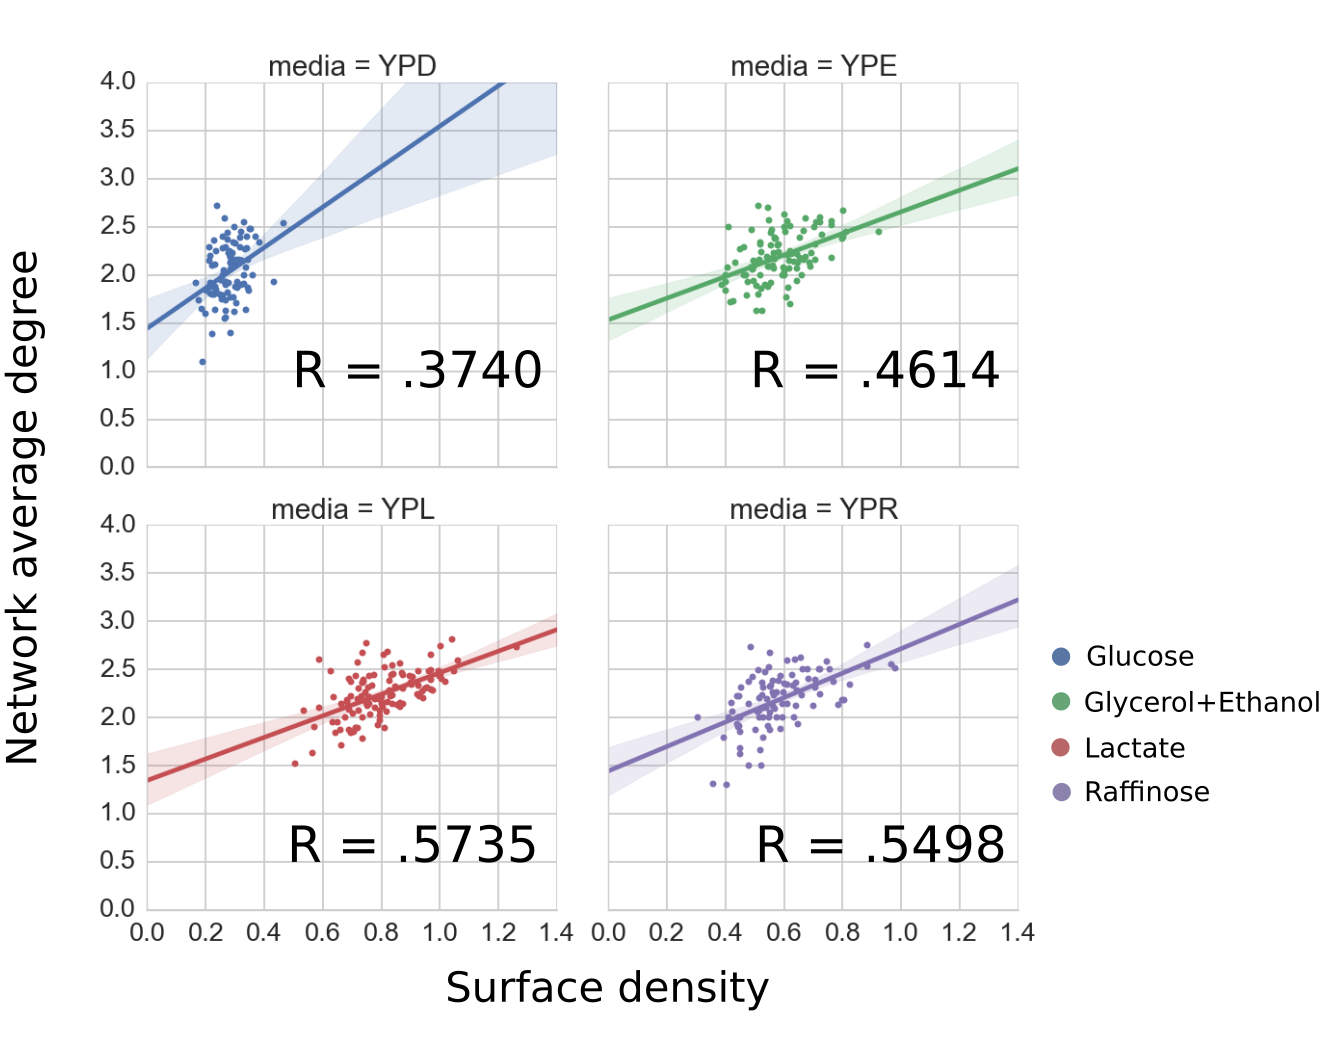
\includegraphics[width=.85\textwidth]{conndense}
    \caption[Network connectivity is positively correlated with mitochondrial surface density]{Network connectivity is positively correlated with mitochondrial surface density.\\Shown here is a plot of the network average degree with the mitochondrial surface density for each cell in different carbon sources. Cells in different carbon sources have different respiration rates which affect the surface density of mitochondria in the cell (\Fref{tab:params}). Mitochondrial networks grown in glucose undergo glucose repression and have the lowest surface density of mitochondria while those in non-fermentable (lactate, glycerol+ethanol) or non repressing fermentable carbon sources (raffinose) undergo aerobic respiration and have increased mitochondrial surface density. The connectivity of the network scales scales positively with the mitochondrial surface density because tubules in a dense mitochondrial network have a higher probability of encountering and forming connections with other tubules. The correlation holds true for other measures of global connectivity (\Fref{tab:glocon}).\\\emph{R value = Pearson correlation coefficient, $p$ value <0.05 that the Pearson correlation score is not significantly different from zero for all conditions.\\Number of cells---Glucose=96, Glycerol+Ethanol=111, Lactate=117, Raffinose=96.}}\label{fig:conndense}
\end{figure}
%
\subsection{Mitochondrial surface density scales with network connectivity}
The first question we address in analyzing functional heterogeneity at the mitochondrial network level is whether mitochondrial surface density and the connectivity of the network are related. In \Fref{fig:conndense} we plot the network average degree against the mitochondrial surface density for each cell in each of the four carbon sources (representing different respiratory conditions as described in \fref{sec:carbon}). The Pearson correlation coefficients show a significant positive correlation between mitochondrial surface density and the average degree of the network. Mitochondrial surface density also scales with other measures of global network connectivity as shown in \Fref{tab:glocon}. This suggest that mitochondrial tubules in cells with a dense mitochondrial network have a higher probability of forming connections with other tubules, simply by having a higher chance of encountering another tubule.
%
\begin{figure}[htp]
	\centering
    \hspace*{.75in}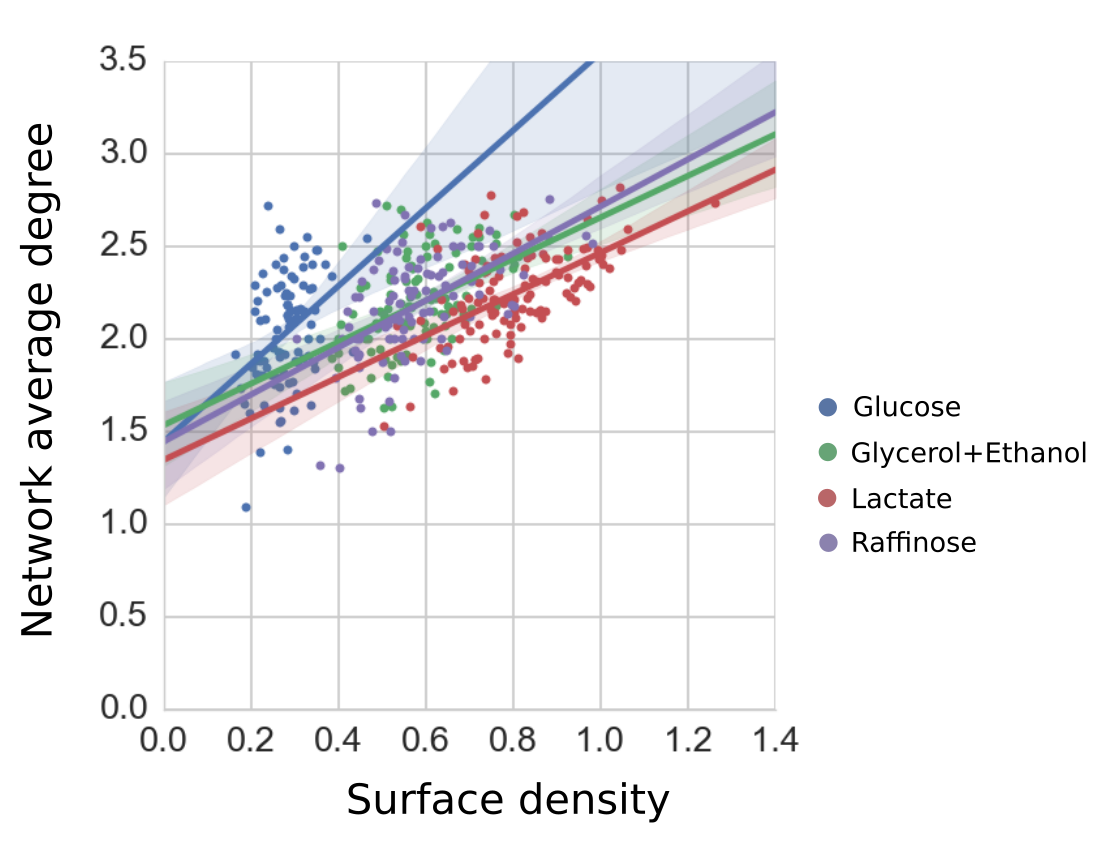
\includegraphics[width=.75\textwidth]{regbeta}
    \caption[Cells in fermentation have a higher regression coefficient for network connectivity--surface density ]{Cells in fermentation have a higher regression coefficient for network connectivity--surface density.\\Shown are the least square regression plots for the relationship between network average degree and surface density, for cells in different carbon sources. The respiration state (fermentation (glucose) or aerobic respiration (non-glucose)) affects the regression coefficient, $\beta$. For a given cell surface density, cells in fermentation display a higher network average degree.}\label{fig:regbeta}
\end{figure}
%

The correlation coefficients in \Fref{tab:glocon} only indicate how linear is the relationship between surface density and global connectivity. When the actual regressions were plotted (\Fref{fig:regbeta}), we see that cells in fermentation (glucose) display a steeper regression slope/coefficient ($\mitbeta$) compared to those in respiration (lactate, glycerol+ethanol, raffinose). This was true as well for the other global connectivity coefficients (not shown). We performed a statistical test on whether there was an interaction between the state of the cell (fermentation/respiration) and their regression coefficient for network average degree--surface density. This is a standard way to test if two different regression coefficients are the same \cite{jacoby_regression}. An interaction that is close to zero indicates that the regression coefficients between two populations are equal. The interaction term ('slope Density.:fermt[T.resp]', \Fref{tab:mytest}) is significantly different from zero ($\mitbeta_{\mathrm{respiration}}$ is -1.33 lower than $\mitbeta_{\mathrm{fermentation}}\,$, $p$ <0.01). Similar results were obtained when using different global connectivity measures (data not shown). This means that cells in fermentation display a higher connectivity for the same surface density compared to cells in respiration. This could indicate that connectivity is regulated in a respiration independent manner as cells in fermentation display network connectivity at a higher level then would be predicted by their surface density values alone (discussed in more detail in \fref{sec:discfive}).

The surface density does not show a strong correlation with measures of centrality or clustering coefficient (\Fref{tab:locon}). A high centrality score indicates the node is a 'hub', i.e. that node is at the intersection of many paths between other pairs of nodes. Our results suggest that nodes do not become more 'central' and the network does not become more of a 'hub-like architecture' as surface density increases.
\subsection{Mitochondrial surface density does not correlate with ΔΨ or connectivity}
We next investigate whether ΔΨ of the network correlates with network connectivity, as it has been observed that larger networks tend to have more fusion events \cite{jakobs_spatial_2003} which requires ΔΨ. Surprisingly we find that there is no correlation between the surface density of mitochondria with the mean cellular ΔΨ (the Pearson correlation coefficient between surface density and ΔΨ was not significantly different from zero, \Fref{fig:dydense}). We also investigated whether ΔΨ correlated with network connectivity (\Fref{tab:dyglo} and \Fref{tab:dylo}) and found no correlations that were significant. This means that a highly connected node (or region of nodes) does not have a different ΔΨ level compared to any other node.
%
\begin{figure}[htp]
	\centering
    \hspace*{.5in}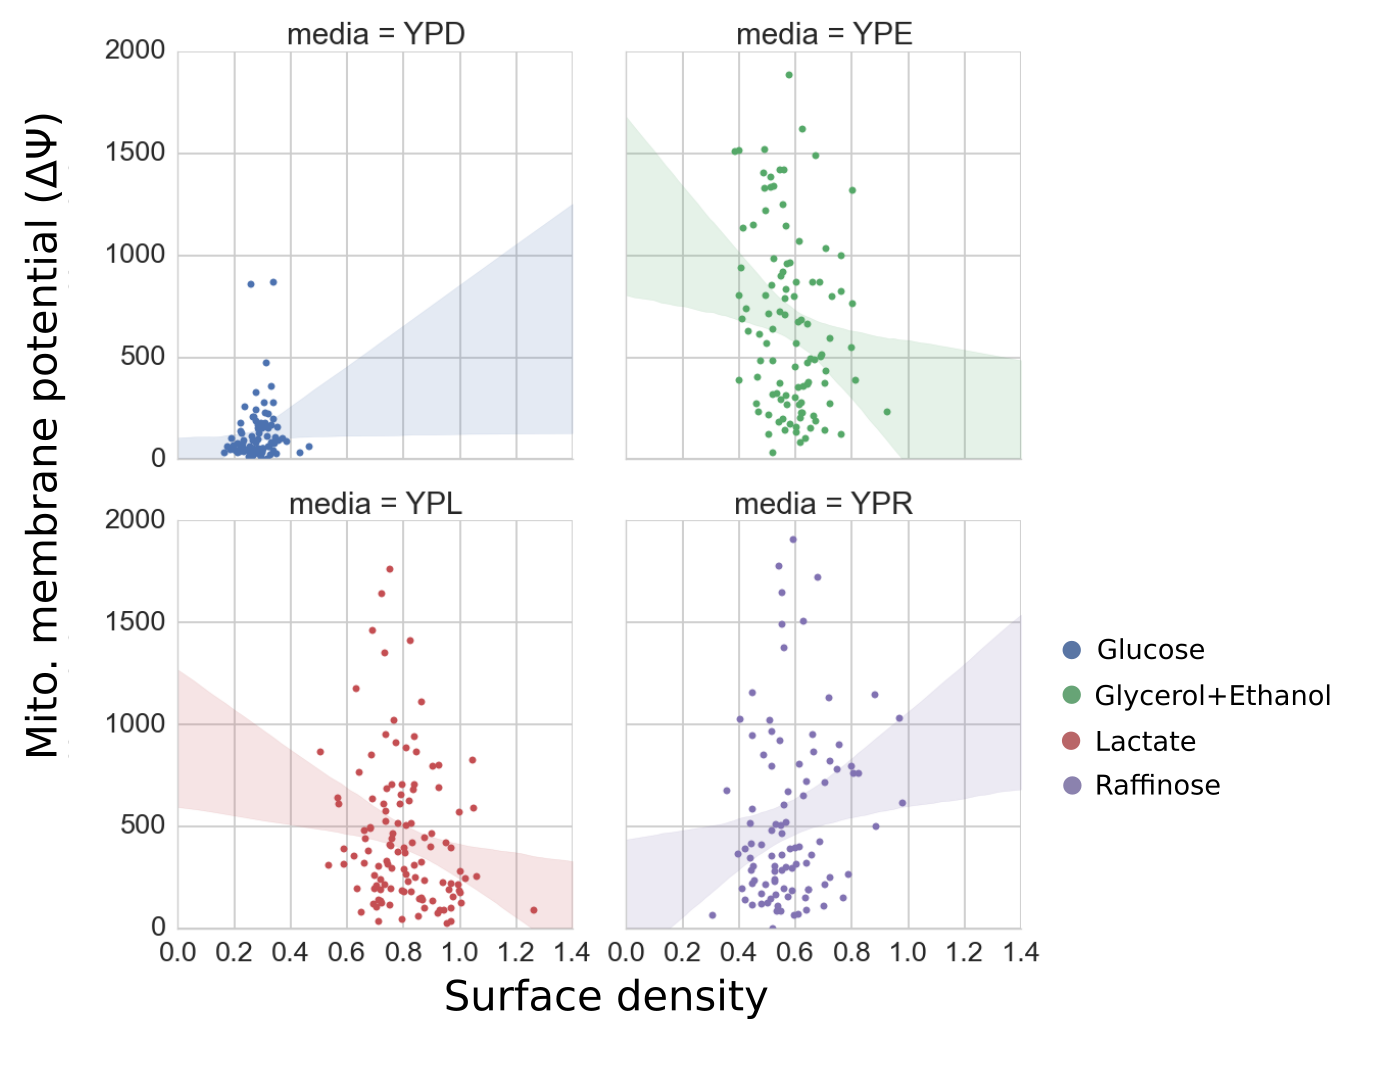
\includegraphics[width=.9\textwidth]{dydense}
    \caption[Mitochondrial membrane potential is not correlated with mitochondrial surface density]{Mitochondrial membrane potential is not correlated with mitochondrial surface density.\\Shown here is a plot between the mean mitochondrial membrane potential (ΔΨ) and mitochondrial surface density for each cell in different carbon sources (see \fref{sec:carbon} for details of the carbon sources). The $p$ value is >0.05, meaning that the Pearson correlation coefficient is not significantly different from zero for all conditions. There was also no clear correlation between ΔΨ and connectivity (\Fref{tab:dyglo} and \Fref{tab:dylo}). We conclude that cellular ΔΨ is independent of the surface density and connectivity of mitochondria in the cell. Changes in the respiration state (glucose vs the others) did not affect the lack of correlation between network connectivity and ΔΨ.}\label{fig:dydense}
\end{figure}
%
\subsection{Mitochondria with similar surface densities do not show a difference in correlation with ΔΨ or connectivity measures}
%
\begin{figure}[htp]
	\centering
    \hspace*{1.25in}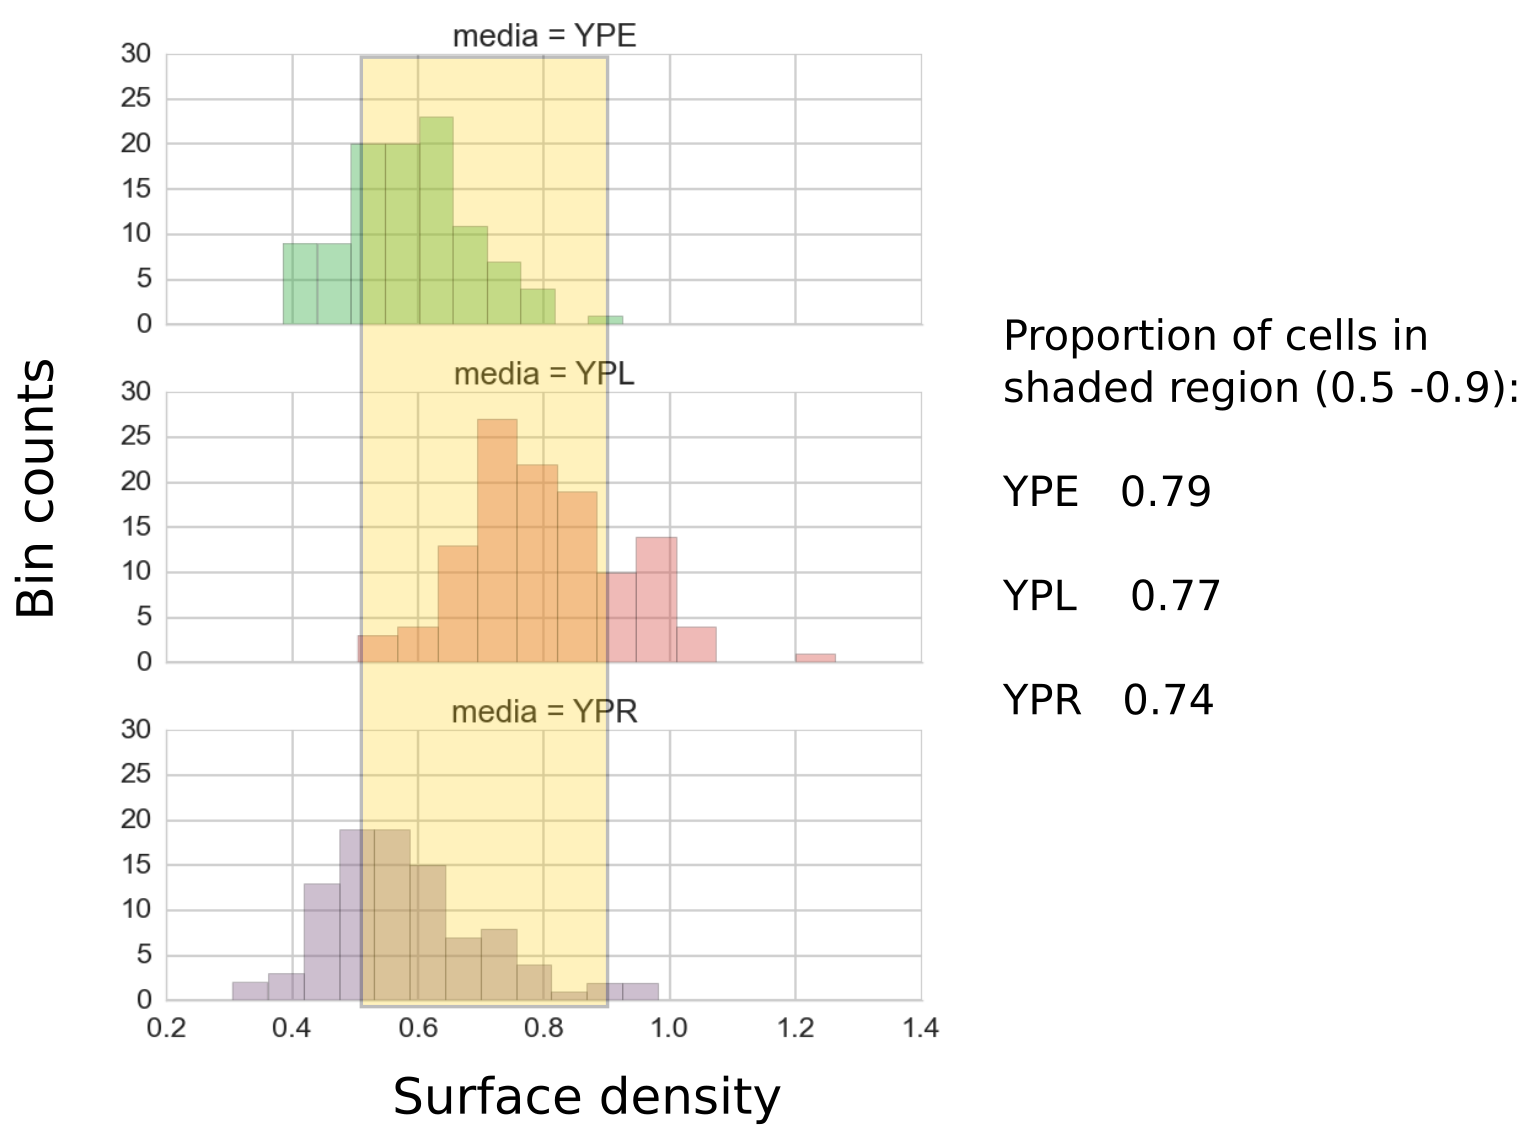
\includegraphics[width=.65\textwidth]{hist}
    \caption[Histogram of cell populations in respiratory conditions based on surface density]{Histogram of cell populations in respiratory conditions based on surface density.\\Variation in surface density in population of cells undergoing aerobic respiration might confound the analysis of ΔΨ with connectivity. To control for this, a subpopulation of the cells (shaded region) with surface density in the range 0.5--0.9 was selected to allow comparisons of ΔΨ and connectivity with similar surface densities of mitochondria. The size of the subpopulations was indicated as a proportion of the total number of cells in the full population.\\\emph{YPE = Glycerol+Ethanol, YPL = Lactate, YPR = Raffinose.}}\label{fig:hist}
\end{figure}
%
%
\begin{figure}[htp]
	\centering
    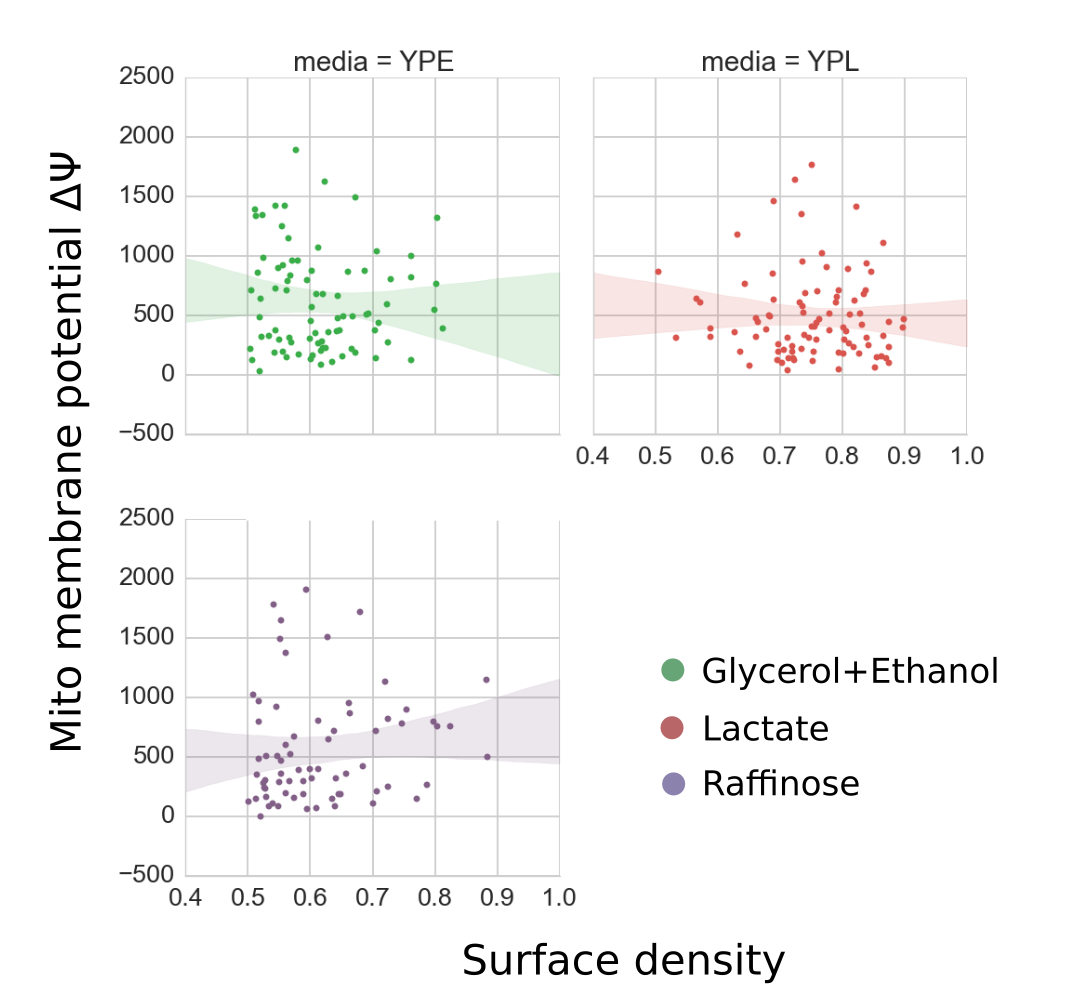
\includegraphics[width=.55\textwidth]{subset}
    \caption[Cells with similar surface density do not show correlation of with surface density]{Mitochondrial membrane potential is not correlated with surface density for subpopulation of cells with surface density in the range 0.5--0.9.\\After taking a subpopulation of cells with similar surface densities (\Fref{fig:hist}) for the three populations undergoing respiration, we found no correlation between ΔΨ and surface density. We also did not find significant correlations between ΔΨ and connectivity measures in the subpopulation (\Fref{tab:glosub}).}\label{fig:subset}
\end{figure}
%
A possible confounding factor when comparing connectivity vs ΔΨ of populations of cells grown in different carbon sources is that they display some variance in their surface density (\Fref{tab:params}). Since connectivity is affected by density, we have to ensure that we are comparing cell populations grown in carbon sources with similar surface densities of mitochondria in order to get a meaningful comparison. We decided to take a subpopulation of cells with a surface density in the range of 0.5--0.9 (\Fref{fig:hist}), ensuring that we had cells with a default higher amount of mitochondrial surface density. There were no cells from the glucose population (YPD) with surface density values in this range. As shown in (\Fref{fig:subset}) there was still no correlation between ΔΨ and mitochondrial surface density.
\subsection{Branchpoint regions have similar ΔΨ to non branchpoint regions}
%
\begin{figure}[htp]
	\centering
    \hspace*{.8in}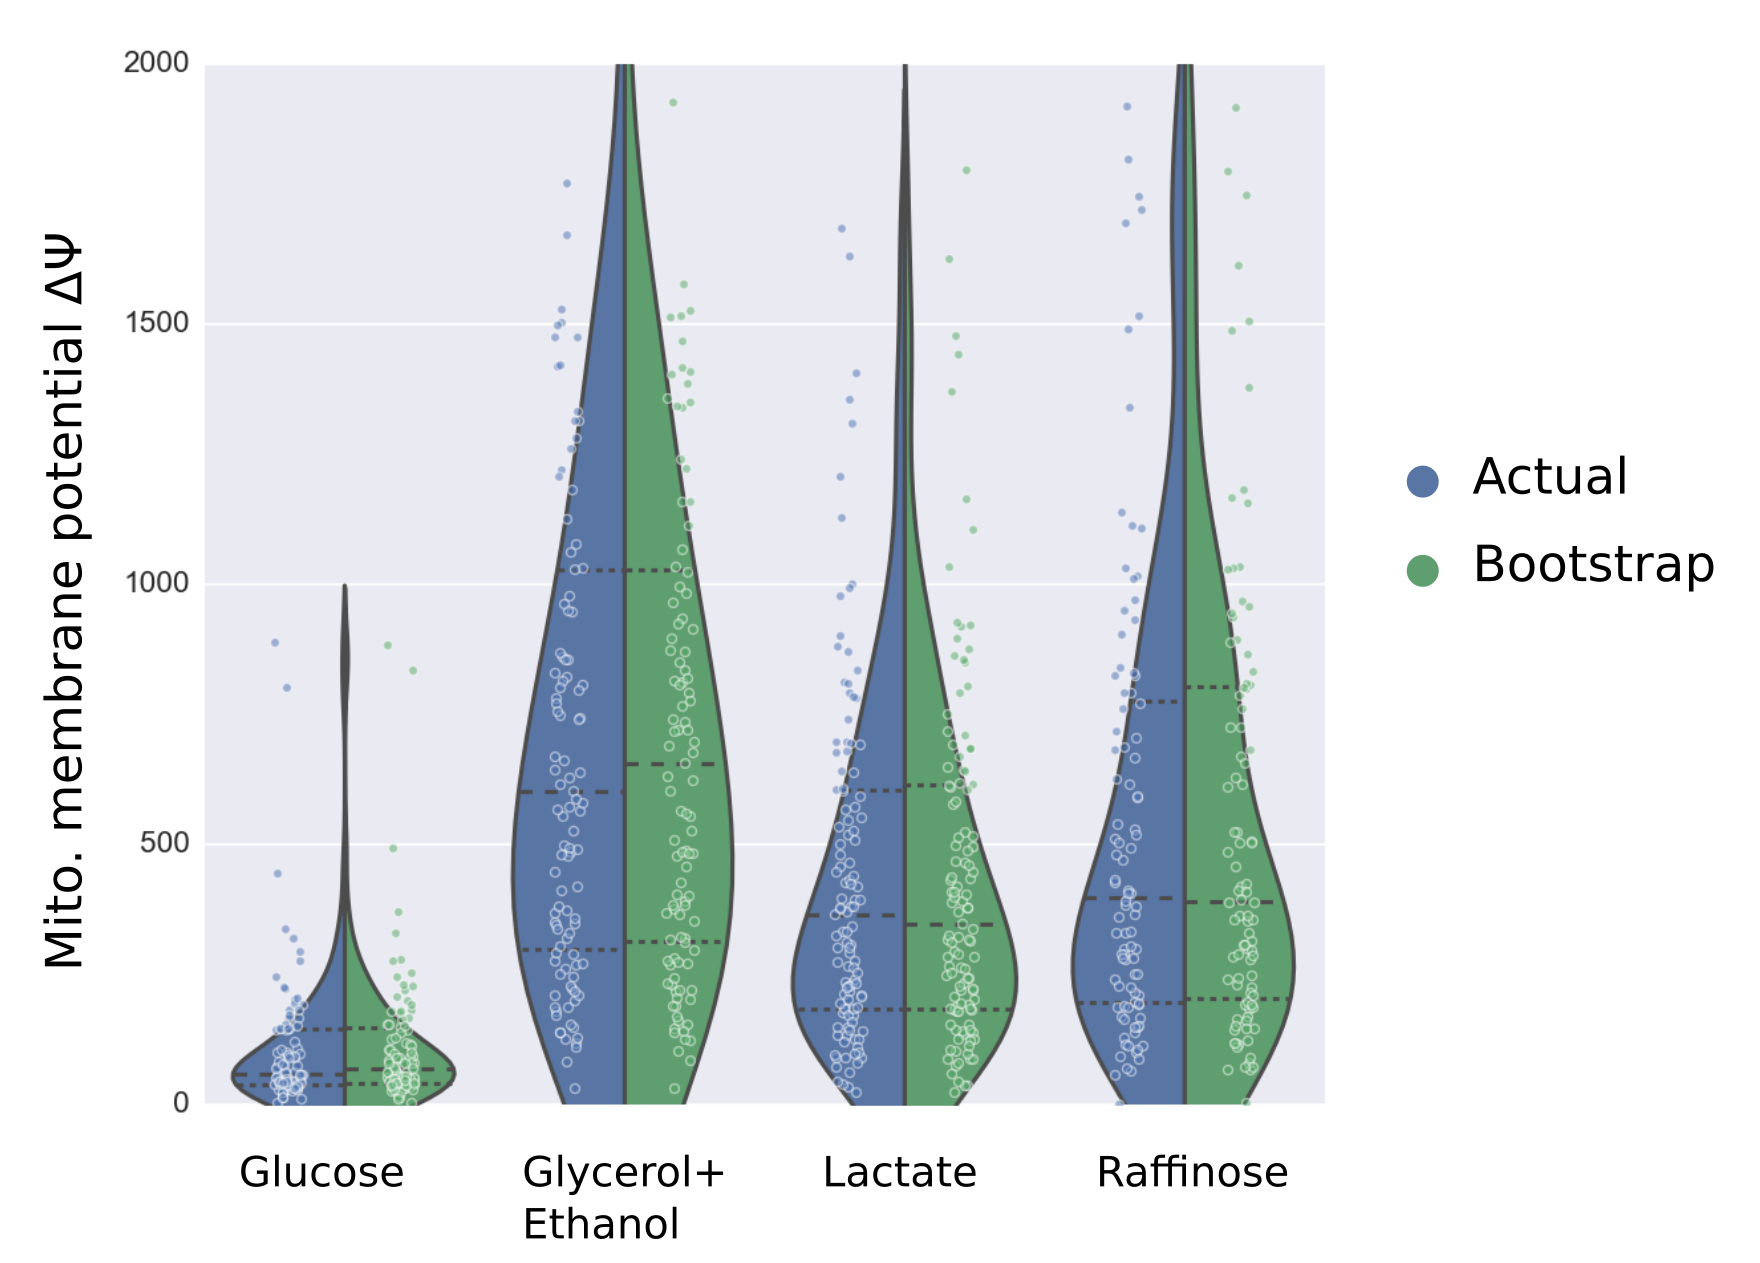
\includegraphics[width=.75\textwidth]{bpoints}
    \caption[Branchpoints do not show a difference in mean mitochondrial membrane potential (ΔΨ) compared to non branchpoints]{Branchpoints do not show a difference in mean mitochondrial membrane potential (ΔΨ) compared to non branchpoints.\\Shown here is the distribution of mean ΔΨ for each branchpoint (blue) or non branchpoint (green) for all mitochondrial networks in a population. To compare branchpoints ΔΨ and non branchpoints ΔΨ, a bootstrapped sampling of voxels that were not in the branchpoints regions was used to estimate the mean ΔΨ of non branchpoint regions. A branchpoint region was defined as a spherical region of radius 300nm centered at a node with degree of three or higher. The sampling population was equal to the number of branchpoints in that cell.\\\emph{Total number of branchpoints---Glucose=1134, Glycerol+Ethanol=1956, Lactate=3507, Raffinose=1623.}}\label{fig:bpoints}
\end{figure}
%
Since branchpoint regions are by definition sites of higher connectivity compared to the rest of the network, we investigated whether regions of mitochondrial tubules near a branching point (within a radius of \SI{300}{\nm}) had different ΔΨ levels compared to non branchpoint regions. We did this via a bootstrap sampling approach to compare branchpoints with equivalent samples of non branchpoints. The blue dots in \Fref{fig:bpoints} show the mean ΔΨ value of all branchpoints in a particular cell. For example for glucose where $N=96$ cells, there are 96 blue dots representing the mean ΔΨ of all branching points in each cell.

There are of course many fewer branchpoint regions compared to non branchpoint regions in a cell. To account for this, for each cell we sampled from the distribution of all non branchpoint voxels (defined as not lying within \SI{300}{\nm} of a branchpoint) in the mitochondrial network to construct a bootstrapped population of 'non-branchpoint' regions. The sampling population was equal to the number of branchpoints in that cell.
The mean of all the bootstrapped 'non-branchpoint' regions was then plotted as a green dot for the cell, and repeated for all cells in all populations (\Fref{fig:bpoints}). As can be seen from the violin plots in the figure, there was no difference in the distributions of ΔΨ between branchpoints and non branchpoints. Statistical testing performed as in \fref{sec:stat} also revealed no significant difference between the branchpoints and non branchpoints. Thus we conclude that branchpoints did not have a different ΔΨ level compared to non branchpoint regions.
\subsection{ΔΨ of isolated mitochondrial fragments are no different from the rest of the network }
%
\begin{figure}[htp]
	\centering
    \hspace*{.5in}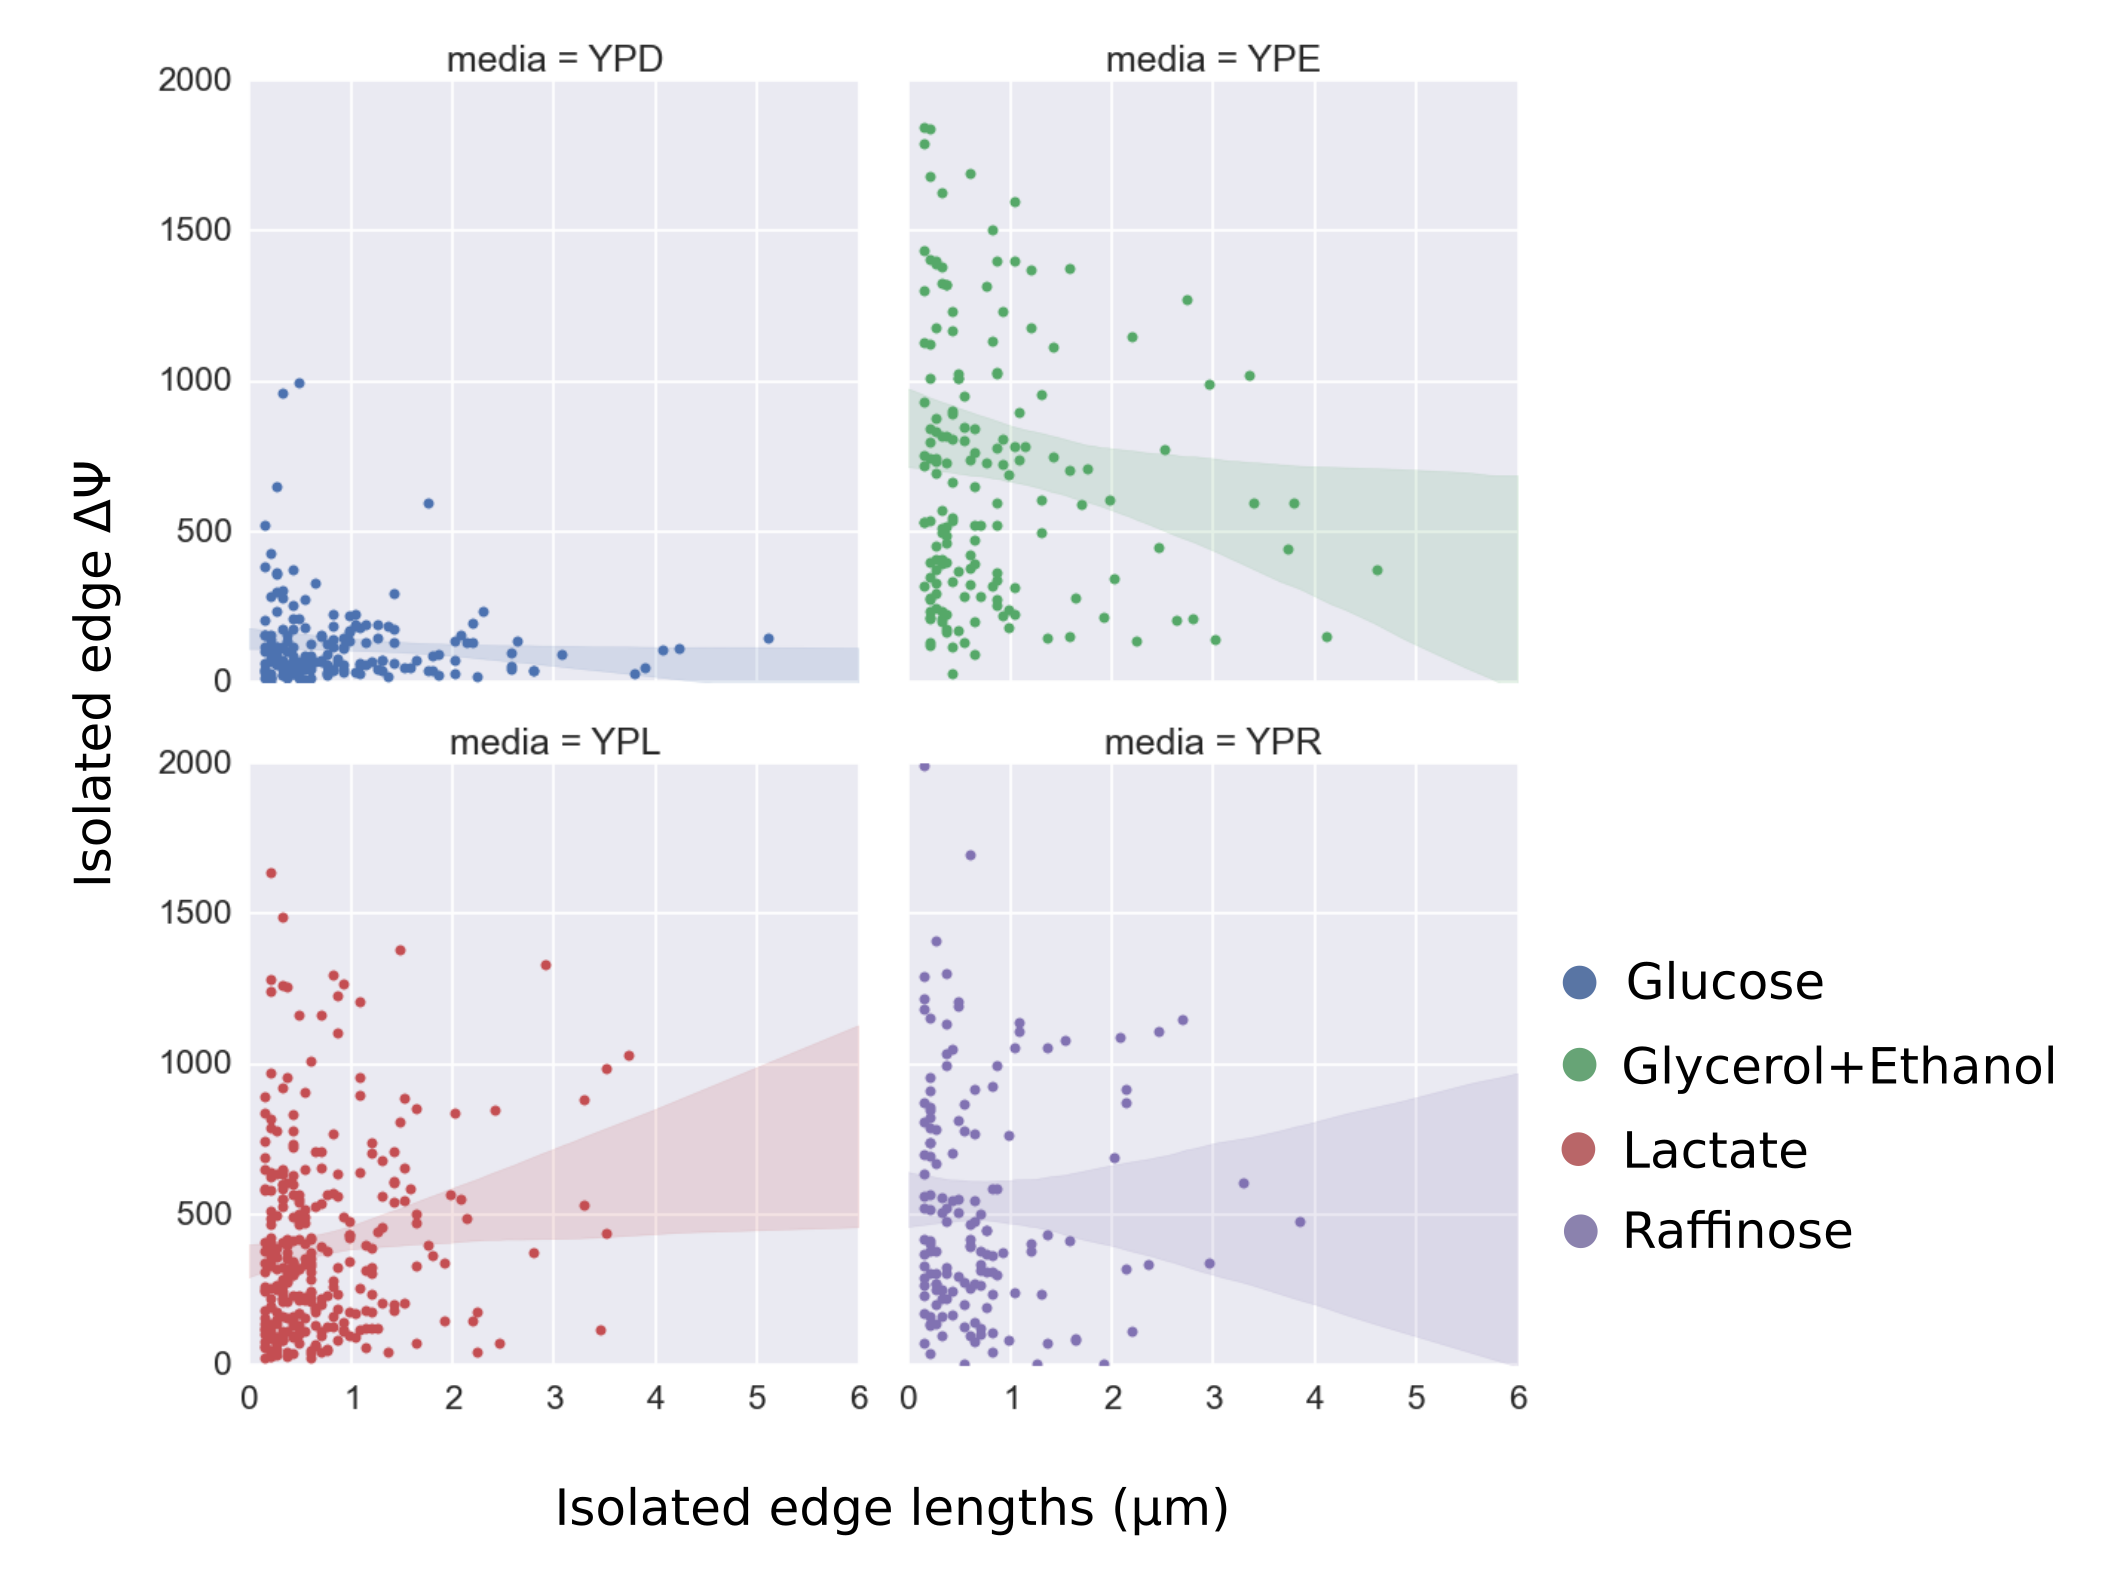
\includegraphics[width=.9\textwidth]{isoedges}
    \caption[Isolated mitochondrial fragments do not show a correlation of size with mitochondrial membrane potential]{Isolated mitochondrial fragments do not show a correlation of size with mitochondrial membrane potential.\\Shown here is plot of the mean ΔΨ vs length of all isolated mitochondrial tubules in each carbon source population. The lack of correlation between fragment ΔΨ and fragment length means that mitophagy selection does not depend on ΔΨ. Previous studies have shown that larger fragments are protected from mitophagy (\cite{rambold_tubular_2011}), hence if mitophagy selection was affected by ΔΨ it would be expected that the large fragments will have a higher overall ΔΨ, based on the assumption that healthier mitochondria are protected from mitophagy.\\\emph{Number of isolated fragments---Glucose=173, Glycerol+Ethanol=169, Lactate=305, Raffinose=148.}}\label{fig:isoedges}
\end{figure}
%
According to the mitochondrial quality control model, damaged mitochondria are targeted for mitophagy. It is also well known that mitophagy rate is correlated with mitochondrial length since small mitochondrial fragments are easier to be processed by the mitophagy machinery \cite{kanki_mitophagy_2008,rambold_tubular_2011}. We investigated whether isolated mitochondrial fragments with short lengths have a lower ΔΨ level, because we expected that on average any isolated fragments of mitochondria that were observed in the network would be those that have lower health/function and therefore be unable to fuse back to the network. We defined an isolated mitochondria in a network as a subgraph with only one edge. We found no correlation between ΔΨ and the length of the isolated mitochondria (\Fref{fig:isoedges}). Furthermore there was no clear clustering of short mitochondrial fragments in the low ΔΨ region, which would be observed if there was a 'threshold' level of functional fitness where short isolated mitochondria are targeted for mitophagy. In addition when we compared the ΔΨ of isolated fragments (regardless of their length) against the rest of the network, there was no difference in their mean ΔΨ (\Fref{fig:isorest}).
%
\begin{figure}[htp]
	\centering
    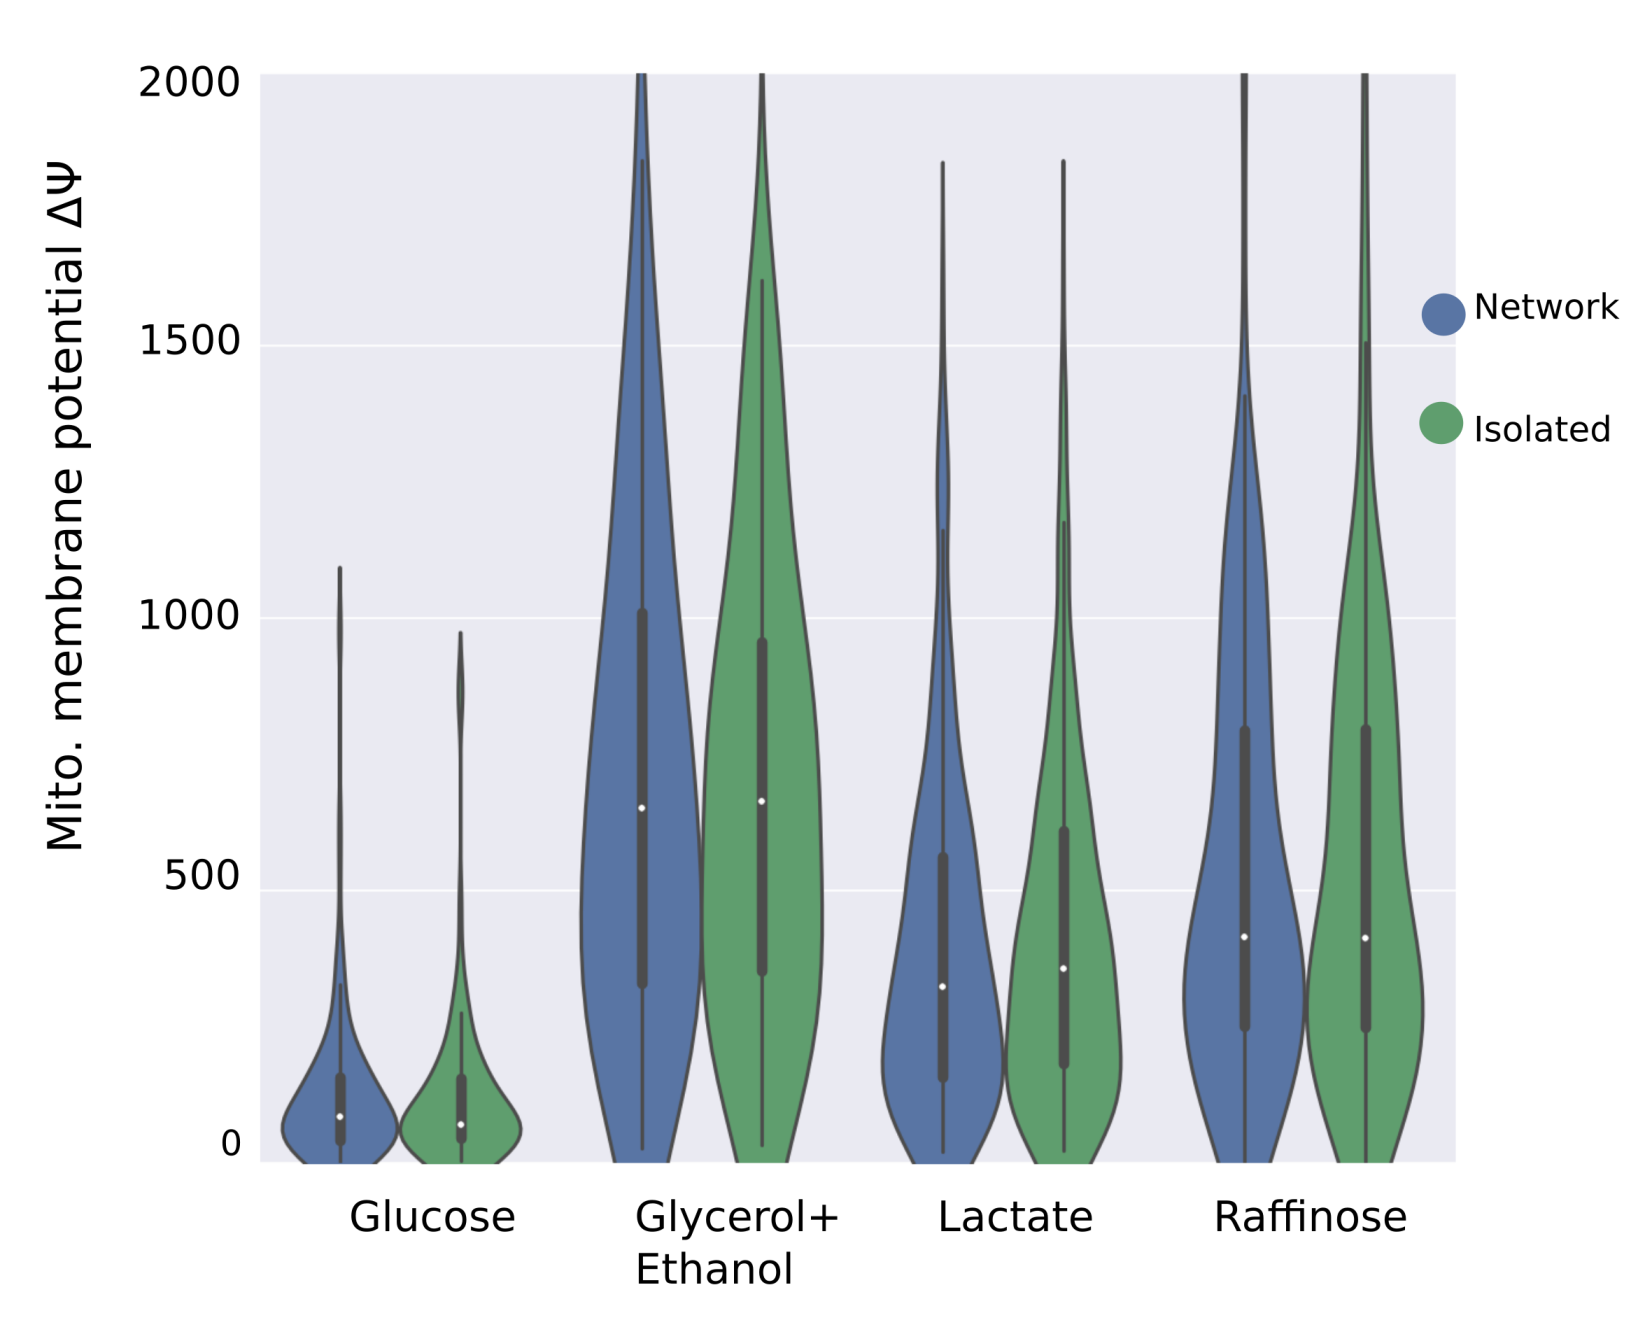
\includegraphics[width=.75\textwidth]{isorest}
    \caption[Isolated mitochondrial fragments do not show a difference in ΔΨ compared to the rest of the mitochondrial network]{Isolated mitochondrial fragments do not show a difference in ΔΨ compared to the rest of the mitochondrial network.\\Shown here is plot of the mean ΔΨ of isolated mitochondrial tubules (green) vs the rest of the connected network (blue) for each population of cells grown in different carbon sources. Isolated fragments do not show a any difference in their mean ΔΨ compared to the network of connected tubules.\\\emph{Number of isolated fragments---Glucose=173, Glycerol+Ethanol=169, Lactate=305, Raffinose=148.}}\label{fig:isorest}
\end{figure}
%

\section{Discussion}\label{sec:discfive}
We consistently found that cells with a higher density of mitochondria also have more connected mitochondrial networks. These results support the idea that mitochondrial tubules in a densely occupied cell surface would have a higher chance to encounter and fuse with another mitochondrial tubule. The three populations that undergo aerobic respiration (glycerol+ethanol, lactate and raffinose) also do not show a difference in their correlation of connectivity with surface density. Thus we conclude that the relationship between network connectivity and amount of mitochondria in the cell is independent of the carbon source as long as it undergoes respiration. Mitochondrial networks undergoing fermentation show a lower correlation between network connectivity and surface density. We found that mitochondrial networks in fermentation have a higher slope for the relationship between network connectivity and surface density. This means that cells in fermentation tend to form more connected networks at a given surface density value compared to those in respiration. As cells in fermentation have lower surface density (\Fref{tab:params}), it might be argued that this tendency for them to form more connected networks compared to respiring cells with the equivalent surface density is to reach a certain level of connectivity regardless of mitochondrial density. However this reasoning is complicated by the fact that cells in fermentation have a statistically significant lower overall connectivity level compared to those in respiration (see columns $\text{β}_{\V{geometric}}\,$, $\text{β}_{\V{topological}}\,$, φ, Pk$_3$ and average degree in \Fref{tab:params}, refer to \Fref{tab:tests} for the statistical test results). Nonetheless, our results imply that network connectivity is an essential feature of mitochondrial networks that is largely independent of respiration state. Results from our lab (data by M.Viana) indicate that one such role is to serve as a substrate to spread and mix mitochondrial content within the network. Simulations of fission/fusion protein mutants show that mitochondrial content mixing occur at a far slower rate compared to wild type cells. This is because wild type cells have network topologies with many more connections that can provide access to content mixing compared to fission/fusion mutants.

According to a model \cite{sukhorukov_emergence_2012} of the relationship between fusion/fission rates and the overall connectivity of the network, the probability $p$ of any two mitochondrial units to be connected are:
\begin{equation}
	\begin{split}
		\begin{aligned}
			&p=\frac{\text{α}_{\V{fusion}}}{\text{α}_{\V{fission}}+\text{α}_{\V{fusion}}} \\
			& \text{α}_{\V{fission}} \text{ and } \text{α}_{\V{fusion}} \text{ are the fission and fusion rates}
		\end{aligned}
	\end{split}
\end{equation}

Based on the model, above a critical value $p_c$ the network will be hyperfused (form a giant connected network with no tubules with free ends). As the global connectivity is higher in respiratory conditions, this implies that mitochondrial networks in respiratory conditions have higher fusion rate or lower fission rate. This suggests that respiration drives the fusion rate higher in order to increase mitochondrial surface density. An example of how fusion rate might be controlled is seen in the regulation of OPA1 processing in mammalian cells. It has been observed that OPA1 is targeted for increased proteolytic processing when ΔΨ is low \cite{ehses_regulation_2009}. This results in a lower overall fusion rate.

We found that ΔΨ did not correlate with either the surface density nor the connectivity of the network. This was surprising because cells with a higher respiration rate (and therefore increased mitochondrial amount) would be expected to have a high mitochondrial bioenergetic state. One possible explanation is that there is no selective fusion, hence no correlation between healthy/high ΔΨ mitochondria and dense/highly connected networks can be observed. However this conclusion goes against the dogma of mitochondrial quality control and would require much more direct evidence to prove this. Another possibility is that the selective fusion threshold is not based on ΔΨ but some other measure of mitochondrial function such as redox state or ROS levels. This hypothesis can be tested by adapting the pipeline described in \Fref{ch:two} to use biomarkers for redox or ROS levels \cite{mcfaline-figueroa_mitochondrial_2011}. The other possibility is that our assumption that highly connected regions were also the sites of higher mitochondrial fusion and fission activity is not true, at least at the global level. However there might still be localized areas of highly connected regions in the network that have higher fusion rates. This would require dynamic data (timelapse imaging) and an automated, reliable way to track fission and fusion sites. Work on this enhancement to MitoGraph is currently ongoing.

We also predicted that branchpoints, which are regions that have undergone fusion would be functionally different (in terms of ΔΨ). However our result indicating that there was no difference in ΔΨ between branchpoints and non branchpoints suggests that there is no functional difference. However without dynamic data we cannot distinguish which branchpoints have higher fusion activity and so cannot conclusively say that there is no functional difference in branchpoints. 

Lastly, we found it surprising that isolated fragments of mitochondria did not exhibit a lower level of ΔΨ. This is because the quality control model states that isolated mitochondria that are unable to fuse back to the network are targetted for mitophagy. Selective fusion means that these isolated fragment would on average be of lower ΔΨ. We further constrained our analysis to small fragments since mitophagy is known to size selective and still did not find a clear clustering of isolated mitochondrial fragments with lower ΔΨ. This suggest that there is no dependence on ΔΨ for mitophagy, which has been suggested in the literature \cite{hoitzing_what_2015}. However it is also possible that the isolated fragments we see are a mixture of fragments that have just undergone fission and have yet to fuse back. Thus we would need dynamic data to observe the mitochondrial fragments that undergo mitophagy and compare their ΔΨ just before undergoing mitophagy to conclusively determine whether mitophagy selects for lower ΔΨ fragments. Alternatively, we can create two populations with different mitophagy rates; a wild type population and a population with either a mitophagy impaired mutant \cite{kanki_atg32_2009} or one with increased fusion rate. In the mitophagy impaired mutant we expect the average ΔΨ to be lower than the wild type ΔΨ as there will be more unhealthy mitochondria in the population that is not mitophagized. Conversely in the population with increased fusion rates, we expect that there will be less unhealthy mitochondria in the population and hence a higher average ΔΨ compared to the wild type population.

In conclusion, we have determined that mitochondria form more connected networks when they are densely packed on the cell surface. However we could not find any evidence that these highly connected and densely packed networks have higher ΔΨ. We also could not find any functional difference in branchpoints or isolated mitochondrial fragments. Therefore we conclude that we will need dynamic data in order to resolve some of these surprising results.
\bigskip

\begin{table}[htp]
\sisetup{round-mode = places,round-precision = 3,table-format=3.3,table-space-text-post=1}
\centering
\caption[ΔΨ, global connectivity, local connectivity and surface density measures of mitochondrial networks in cells grown in various carbon sources.]{ΔΨ, global connectivity, local connectivity and surface density measures of mitochondrial networks in cells grown in various carbon sources.\\ $*\ p$<0.05 for the null hypothesis test that YPD is not significantly different from YPE, YPL and YPR, using rank sum test with multiple testing correction as detailed in \fref{sec:stat}. A list of tables for the statistical testing between conditions is included in the Appendix section (\Fref{tab:tests}).}
\footnotesize
\begin{tabular}{lSSSS}
\toprule
Carbon source &  {\parbox{1in}{\centering{ΔΨ (a.u.)}}} & \text{Surface Density}&$\text{β}_{\V{geometric}}$ & $\text{β}_{\V{topological}}$\\
\midrule
YPD (Glucose) & 114.2* &0.2812&0.6738* & 0.6842*\\
YPE (Ethanol +Glycerol) & 661.7 &0.5855&0.7851 & 0.7806\\
YPL (Lactate) & 443.5 & 0.8046&0.8099 & 0.8072\\
YPR (Raffinose) & 534.7 & 0.5812&0.7945 & 0.7970\\
\midrule
Carbon source & {\parbox{1in}{\centering{Pk$_3$}}}  & \text{Average degree} & {\parbox{1in}{\centering{Edge numbers}}}& {\parbox{1in}{\centering{φ}}} \\
\midrule
YPD (Glucose) & 0.4861* & 2.0352* & 24.7&0.6175*\\
YPE (Ethanol +Glycerol) & 0.5552 & 2.1903 & 34.4&0.7233\\
YPL (Lactate) & 0.5763 & 2.2466 & 58.2&0.7513\\
YPR (Raffinose) & 0.5567 & 2.1829 & 33.1&0.7422\\
\midrule
Carbon source & {\parbox{1in}{\centering{Betweenness centrality}}} & {\parbox{1in}{\centering{Near. neigh. degree}}} & {\parbox{1in}{\centering{Closeness centrality}}} & {\parbox{1in}{\centering{Clustering coefficient}}}\\
\midrule
YPD (Glucose) & 0.1149 & 2.3033* & 0.2165 &0.1163\\
YPE (Ethanol +Glycerol) & 0.1220 & 2.5151 & 0.2086&0.1053\\
YPL (Lactate) & 0.1027 & 2.6351 & 0.1559&0.0987\\
YPR (Raffinose) & 0.1355 & 2.5193 & 0.2125&0.1132\\
\bottomrule
\end{tabular}
\label{tab:params}
\end{table}
%

\begin{table}[htp]
\sisetup{round-mode = places,round-precision = 3,table-format=1.3,table-space-text-post=1}
\centering
\caption[Correlation of surface density with global connectivity]{Correlation of surface density with global connectivity.\\$p$<0.05 for all values in the table. The null hypothesis test was that the correlation coefficients were not significantly different from 0.}
\footnotesize
\begin{tabular}{p{2in}SSSS}
\toprule
Pearson correlation score of surface density with & \text{YPD} & \text{YPE} & \text{YPL}&\text{YPR}\\
\midrule 
Average degree & 0.3740 & 0.4614 & 0.5735&0.5498 \\ 
$\text{β}_{\V{geometric}}$& 0.3227 & 0.2607 & 0.4495&0.3803 \\ 
$\text{β}_{\V{topological}}$ & 0.2874 & 0.2864 & 0.4280&0.4126 \\ 
Edge numbers & 0.3665 & 0.3811 & 0.4846&0.5006 \\ 
\text{φ} & 0.3290 & 0.3302 & 0.4756&0.4551 \\ 
Pk$_3$ & 0.3889 & 0.4214 & 0.5856&0.5426 \\ 
\bottomrule
\end{tabular}
\label{tab:glocon}
\end{table}
%

\begin{table}[htp]
\sisetup{round-mode = places,round-precision = 3,table-format=1.3,table-space-text-post=1}
\centering
\caption[Correlation of surface density with local connectivity]{Correlation of surface density with local connectivity. \\$*\ p$<0.05 for the null hypothesis test that the correlation coefficients were not significantly different from 0.}
\footnotesize
\begin{tabular}{p{2in}SSS[table-format=-1.3,table-space-text-post=1]S}
\toprule
Pearson correlation score of surface density with & \text{YPD} & \text{YPE} & \text{YPL}&\text{YPR}\\
\midrule 
Average degree & 0.3740 & 0.4614 & 0.5735&0.5498 \\ 
Betweenness centrality & 0.2030 & 0.1171 & 0.2280&0.0787 \\ 
Closeness centrality & 0.0437 & 0.0576 & 0.1606&0.0749 \\ 
Clustering coefficient & 0.1575 & 0.0084 & -0.0315&0.1113 \\ 
Nearest neighbor degree & 0.4590* & 0.4559* & 0.5043*&0.5303* \\ 
\bottomrule
\end{tabular}
\label{tab:locon}
\end{table}
%

\begin{table}[htp]
\sisetup{round-mode = places,round-precision = 3,table-format=-1.3,table-space-text-post=1}
\centering
\caption[Correlation of ΔΨ with global connectivity and surface density]{Correlation of ΔΨ with global connectivity and surface density. No significant correlations were found.}
\footnotesize
\begin{tabular}{p{2in}SSSS}
\toprule
Pearson correlation score of ΔΨ with & \text{YPD} & \text{YPE} & \text{YPL}&\text{YPR}\\
\midrule 
Surface density & 0.1523 & -0.2319 & -0.2203&0.2058 \\ 
Average degree & -0.0430 & -0.0938 & 0.1193&0.0452 \\ 
$\text{β}_{\V{geometric}}$ & -0.0026 & -0.1545 & 0.0222&0.0591 \\ 
$\text{β}_{\V{topological}}$ & 0.0112 & -0.1147 & 0.0447&0.0605 \\ 
Edge numbers & 0.0260 & -0.1098 & -0.2652&-0.0831 \\ 
\text{φ}& -0.0073 & -0.0915 & 0.0606&0.0672 \\ 
\bottomrule
\end{tabular}
\label{tab:dyglo}
\end{table}
%

\begin{table}[htp]
\sisetup{round-mode = places,round-precision = 3,table-format=-1.3,table-space-text-post=1}
\centering
\caption[Correlation of ΔΨ with local connectivity]{Correlation of ΔΨ with local connectivity. No significant correlations were found.}
\footnotesize
\begin{tabular}{p{2in}SSS[table-format=1.3,table-space-text-post=1]S[table-format=1.3,table-space-text-post=1]}
\toprule
Pearson correlation score of ΔΨ with & \text{YPD} & \text{YPE} & \text{YPL}&\text{YPR}\\
\midrule 
Betweenness centrality & -0.0258 & -0.1214 & 0.0599&0.0801 \\ 
Closeness centrality & -0.0083 & 0.0001 & 0.2492&0.1567 \\ 
Clustering coefficient & 0.0233 & -0.1632 & 0.2467&0.0519 \\ 
Nearest neighbor degree & 0.0411 & 0.0133 & 0.0840&0.0044 \\ 
\bottomrule
\end{tabular}
\label{tab:dylo}
\end{table}
%

\begin{table}[htp]
\sisetup{round-mode = places,round-precision = 3,table-format=1.3,table-space-text-post=1}
\centering
\caption[Correlation of surface density with global connectivity for the subpopulation of cells with surface density in the range 0.5--0.9]{Correlation of surface density with global connectivity for the subpopulation of cells with surface density in the range 0.5--0.9.\\$*\ p$<0.05 for the null hypothesis test that the correlation coefficients were not significantly different from 0.}
\footnotesize
\begin{tabular}{p{2in}S[table-format=2.0]SSS}
\toprule
Pearson correlation score of surface density with & \text{YPD} & \text{YPE} & \text{YPL}&\text{YPR}\\
\midrule 
Average degree & NA & 0.3816* & 0.4217*&0.4419* \\ 
$\text{β}_{\V{geometric}}$& NA & 0.0873 & 0.3926*&0.3123*\\ 
$\text{β}_{\V{topological}}$ & NA & 0.0896 & 0.3514*&0.3564* \\ 
Edge numbers & NA & 0.3066* & 0.4571*&0.3198*\\ 
\text{φ} & NA & 0.1203 & 0.3595*&0.3880*\\ 
Pk$_3$ & NA & 0.3117* & 0.4421*&0.4190* \\ 
\bottomrule
\end{tabular}
\label{tab:glosub}
\end{table}
%

\begin{table}[htp]
\sisetup{round-mode = places,round-precision = 3,table-format=-1.3,table-space-text-post=1}
\centering
\caption[Correlation of surface density with local connectivity for the subpopulation of cells with surface density in the range 0.5--0.9]{Correlation of surface density with local connectivity for the subpopulation of cells with surface density in the range 0.5--0.9.\\$*\ p$<0.05 for the null hypothesis test that the correlation coefficients were not significantly different from 0.}
\footnotesize
\begin{tabular}{p{2in}S[table-format=2.0]SSS[table-format=1.3,table-space-text-post=1]}
\toprule
Pearson correlation score of surface density with & \text{YPD} & \text{YPE} & \text{YPL}&\text{YPR}\\
\midrule 
Betweenness centrality & NA & -0.0179 & 0.2081*&0.0569 \\ 
Closeness centrality & NA & -0.0161 & 0.0190&0.1102 \\ 
Clustering coefficient & NA & 0.1367 & -0.0097&0.0808 \\ 
Nearest neighbor degree & NA & 0.3955* & 0.4003*&0.4978*\\ 
\bottomrule
\end{tabular}
\label{tab:losub}
\end{table}
















